\documentclass{article}
\usepackage[utf8x]{inputenc}
\usepackage{ucs}
\usepackage{amsmath} 
\usepackage{amsfonts}
\usepackage{upgreek}
\usepackage[english,russian]{babel}
\usepackage{graphicx}
\usepackage{float}
\usepackage{textcomp}
\usepackage{hyperref}
\usepackage{geometry}
  \geometry{left=2cm}
  \geometry{right=1.5cm}
  \geometry{top=1cm}
  \geometry{bottom=2cm}
\usepackage{tikz}
\usepackage{ccaption}
\usepackage{multicol}


\usepackage{listings}


\begin{document}
\pagestyle{plain}
\lstset{
  language=C,                % choose the language of the code
  basicstyle=\linespread{1.1}\ttfamily,
  columns=fixed,
  fontadjust=true,
  basewidth=0.5em,
  keywordstyle=\color{blue}\bfseries,
  commentstyle=\color{gray},
  stringstyle=\ttfamily\color{orange!50!black},
  showstringspaces=false,
  numbersep=5pt,
  numberstyle=\tiny\color{black},
  numberfirstline=true,
  stepnumber=1,                   % the step between two line-numbers.        
  numbersep=10pt,                  % how far the line-numbers are from the code
  backgroundcolor=\color{white},  % choose the background color. You must add \usepackage{color}
  showstringspaces=false,         % underline spaces within strings
  captionpos=b,                   % sets the caption-position to bottom
  breaklines=true,                % sets automatic line breaking
  breakatwhitespace=true,         % sets if automatic breaks should only happen at whitespace
  xleftmargin=.2in,
  extendedchars=\true,
  keepspaces = true,
}
\lstset{literate=%
   *{0}{{{\color{red!20!violet}0}}}1
    {1}{{{\color{red!20!violet}1}}}1
    {2}{{{\color{red!20!violet}2}}}1
    {3}{{{\color{red!20!violet}3}}}1
    {4}{{{\color{red!20!violet}4}}}1
    {5}{{{\color{red!20!violet}5}}}1
    {6}{{{\color{red!20!violet}6}}}1
    {7}{{{\color{red!20!violet}7}}}1
    {8}{{{\color{red!20!violet}8}}}1
    {9}{{{\color{red!20!violet}9}}}1
}

\title{Семинар \#5: Структуры. Классные задачи.\vspace{-5ex}}\date{}\maketitle

\section*{Часть 1: Основы структур}

Структуры служат для объединения нескольких типов в один. В примере ниже был создан новый тип под названием \texttt{struct point}. Переменные этого типа будут содержать внутри себя 2 значения типа \texttt{float}.
\begin{lstlisting}
#include <stdio.h>

struct point {
    float x, y;
}; // <--------------------------- Не забудьте тут точку с запятой!

int main() {
    struct point a = {2.1, 4.3};
    a.x = 7.8;
    printf("(%f, %f)", a.x, a.y);
}
\end{lstlisting}

\subsection*{Операции со структурами}
\begin{enumerate}
\item При создании структуры её элементы можно инициализировать с помощью фигурных скобочек.
\begin{lstlisting}
struct point a = {2.1, 4.3};
\end{lstlisting}
Однако нельзя таким образом присваивать
\begin{lstlisting}
a = {5.6, 7.8}; // Ошибка, так можно только инициализировать
\end{lstlisting}
\item Доступ к элементу структуры осуществляется с помощью оператора точка
\begin{lstlisting}
a.x = 5.6;
a.y = 7.8;
\end{lstlisting}
\item Структуры можно присваивать друг другу. При этом происходит побайтовое копирование содержимого одной структуры в другую.
\begin{lstlisting}
struct point b;
b = a;
\end{lstlisting}
\end{enumerate}

\subsection*{Массив структур}
Структуры, как и обычные переменные, можно хранить в массивах. В примере ниже создан массив под названием \texttt{array}, содержащий в себе 2 точки.
\begin{lstlisting}
#include <stdio.h>
struct point {
    float x, y;
};
int main() {
    struct point array[2] = {{2.1, 4.3}, {7.0, 3.1}};
    array[1].x = 1.8;
    printf("(%f, %f)", array[0].x, array[0].y);
}
\end{lstlisting}

\subsection*{Задачи}
\begin{itemize}
\item Описать структуру \texttt{struct date}, с полями: \texttt{day}, \texttt{month} и \texttt{year}. 
\item Объявить и инициализировать переменную \texttt{a} типа \texttt{struct date} в функции \texttt{main}.
\item Объявить и инициализировать массив дат под названием \texttt{holidays} следующими значениями \texttt{31.12.2021}, \texttt{8.3.2022} и \texttt{9.5.2022}.
\item Напечатать содержимое массива \texttt{holidays} на экран с помощью цикла в следующем виде:
\begin{verbatim}
31.12.2021
08.03.2022
09.05.2022
\end{verbatim}

\end{itemize}

\subsection*{Передача структуры в функцию}
Структуры можно передавать в функции и возвращать из функций также как и обычные переменных. При передаче в функцию происходит полное копирование структуры и функция работает уже с копией структуры. При возвращении из функции также происходит копирование. Для того чтобы избежать лишние копирования нужно передавать структуру по указателю (об этом -- в части 3).

\begin{lstlisting}
#include <stdio.h>

struct point {
    float x, y;
};
void print_point(struct point a) {
    printf("(%f, %f)", a.x, a.y);
}
struct point add_points(struct point a, struct point b) {
    struct point result;
    result.x = a.x + b.x;
    result.y = a.y + b.y;
    return result;
}
int main() {
    struct point a = {2.1, 4.3}, b = {6.7, 8.9};
    struct point c = add_points(a, b);
    print_point(c);
}
\end{lstlisting}

\subsection*{Задачи}
\begin{itemize}
\item Написать функцию \texttt{void print\_date(struct date a)} для печати этой структуры в формате \texttt{DD.MM.YYYY}. Используйте модификатор \texttt{\%02d}. Вызовите эту функцию из main, чтобы напечатать все содержимое \texttt{holidays}.

\item Написать функцию \texttt{struct date pushkin\_birthday()} которая создаёт дату, соответствующую дню рождения А. С. Пушкина (6 июня 1799 года) и возвращает её. Протестируйте эту функцию в \texttt{main}.

\item Написать функцию \texttt{struct date create\_date(int day, int month, int year)} которая создаёт дату, по трём переданным в функцию числам  и возвращает её. Протестируйте эту функцию в \texttt{main}.


\item Написать функцию \texttt{struct date next\_day(struct date a)} которая увеличивает значение даты на один день и возвращает эту структуру. Для простоты не учитываем високосные года и считаем, что в феврале всегда 28 дней. Вызовите эту функцию из \texttt{main}, чтобы увеличить значение даты \texttt{holidays[0]} на 1 день.
\end{itemize}
\newpage
\section*{Часть 2: Структуры содержащие более сложные типы данных}
Структуры могут содержать в себе не только базовые типы данных, но и более сложные типы, такие как массивы (в том числе строки), указатели, а также другие структуры.\\
Пример программы, в которой описывается структура для удобной работы с объектами Книга (\texttt{struct book}).
\begin{lstlisting}
#include <stdio.h>
#include <string.h>

struct book {
    char title[50];
    int pages;
    float price;
};
void print_book(struct book b) {
    printf("Book info:\n");
    printf("Title: %s\nPages: %d\nPrice: %g\n\n", b.title, b.pages, b.price);
}
int main() {
    // Создаём книгу и печатаем её:
    struct book a = {"The Martian", 10, 550.0};
    print_book(a);
    
    // Меняем количество страниц книги и её название и снова печатаем её
    a.pages = 369;
    strcpy(a.title, "The Catcher in the Rye");
    print_book(a);
    
    // Пример работы с массивом структур
    struct book scifi_books[10] = {{"Dune", 300, 500.0}, {"Fahrenheit 451", 400, 700.0},
							 {"Day of the Triffids", 304, 450.0}};
    scifi_books[2].price = 2000.0;
    print_book(scifi_books[2]);
}
\end{lstlisting}


\subsection*{Задачи:}
\begin{itemize}
\item Описать структуру \texttt{struct movie} с полями: 
\begin{itemize}
\item \texttt{title} -- название фильма (строка длиной не более 50 символов).
\item \texttt{running\_time} -- длительность в минутах (\texttt{int})
\item \texttt{rating} -- оценка на Кинопоиске (\texttt{float})
\item \texttt{release\_date} -- дата выхода (используйте структуру \texttt{Date}).
\end{itemize}
\item Объявить переменную типа \texttt{struct movie} в функции \texttt{main} и инициализировать её следующими значениями:\\
\texttt{title -- ``Joker'', running\_time -- 122, rating -- 7.98, release\_date -- \{3, 10, 2019\}}.
\item В новых строках изменить рейтинг и месяц выхода фильма. Используйте оператор точка.
\item Написать функцию \texttt{void print\_movie(struct movie m)} и вызвать её в функции \texttt{ main()}.
\item Написать функцию \texttt{struct movie get\_titanic()} которая будет возвращать структуру с полями \texttt{title -- ``Titanic'',  running\_time -- 194, rating -- 8.4, release\_date -- \{1, 11, 1997\}}. Вызовите эту функцию из \texttt{main} и напечатайте результат возвращаемого значения.
\item Объявить и инициализировать массив, содержащий 10 различных фильмов. Решение этой задачи есть ниже и в файле \texttt{movie\_array\_init.txt}. Просто скопируйте код.
\item В новой строке изменить день выхода фильма \texttt{Pulp Fiction} с 19-го мая на 21-е мая.
\item Написать функцию \texttt{print\_movie\_array(struct movie array[], int size)}, которая бы печатала массив структур \texttt{Movie} и вызвать её в функции \texttt{main()}.
\item Написать функцию, которая по массиву фильмов находит средний рейтинг. Протестируйте её в \texttt{main}.

\item \textbf{Сортировка структур:} Одна из простейших сортировок - это сортировка выбором:
\begin{lstlisting}
void selection_sort(int array[], int size) {
    for (int j = 0; j < size; j++){
        // Находим индекс минимального элемента на отрезке [j:n-1]
        int min_index = j;
        for (int i = j + 1; i < size; i++) {
            if (array[i] < array[min_index]) {
                min_index = i;
            }
        }
		
        // Меняем местами элемент номер j и минимальный элемент
        int temp = array[j];
        array[j] = array[min_index];
        array[min_index] = temp;
    }
}
\end{lstlisting}
Видоизмените эту сортировку так, чтобы она сортировала фильмы по рейтингу (от большего к меньшему). Помните, что структуры можно присваивать целиком, а не поэлементно.
\item \textbf{Сортировка по алфавиту:} Отсортируйте структуры по их названию в алфавитном порядке. Используйте функцию \texttt{strcmp} из \texttt{string.h}. Функция \texttt{strcmp(a, b)} возращает \texttt{0}, если строки равны, отрицательное число если строка \texttt{a} меньше, чем строка \texttt{b} и положительное число, если строка \texttt{a} больше, чем \texttt{b}. 
\end{itemize}

\begin{lstlisting}
struct movie array[10] = {{"The Godfather", 175, 8.735, {14, 3, 1972}},
                          {"The Shawshank Redemption", 142, 9.112, {10, 9, 1994}},
                          {"Fight Club", 175, 8.651, {10, 9, 1999}},
                          {"The Matrix", 131, 8.491, {24, 3, 1999}},
                          {"Pulp Fiction", 154, 8.620, {19, 5, 1994}},
                          {"Citizen Kane", 119, 7.826, {1, 5, 1941}},
                          {"A Clockwork Orange", 137, 7.959, {19, 12, 1971}},
                          {"2001: A Space Odyssey", 149, 7.988, {2, 4, 1968}},
                          {"Finding Nemo", 175, 7.862, {30, 05, 2003}},
                          {"Vzlomat blogerov", 90, 1.029, {10, 11, 2016}}};
\end{lstlisting}

\newpage
\section*{Часть 3: Указатели на структуры:}
Указатель на структуру хранит адрес первого байта структуры. Для доступа к полям структуры по указателю нужно сначала этот указатель разыменовать, а потом использовать: \texttt{(*p).price}. Для удобства был введён оператор стрелочка \texttt{->}, который делает то же самое: \texttt{p->price}.
\begin{multicols}{2}
\begin{lstlisting}
#include <stdio.h>

struct book {
    char title[50];
    int pages;
    float price;
};
int main() {
    struct book a = {"The Martian",277,540};
    struct book* p = &a;
    // Три способа доступа к полю:
    a.price += 10;
    (*p).price += 10;
    p->price += 10;
}
\end{lstlisting}

\vfill\null
\columnbreak

\begin{center}
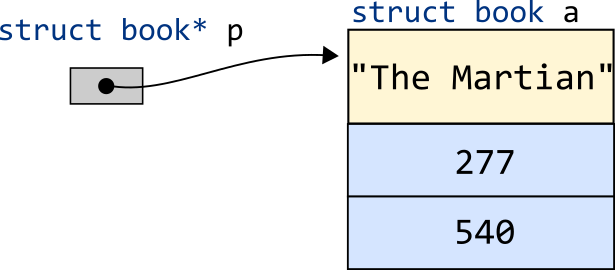
\includegraphics[scale=0.6]{../images/structpointer2.png}
\end{center}
\end{multicols}

\begin{itemize}
\item Измените первую букву поля \texttt{title} структуры, используя только указатель \texttt{p}.
\end{itemize}

\subsection*{Передача по значению}
При обычной передаче в функцию всё содержимое копируется. Функция работает с копией.
\begin{lstlisting}
#include <stdio.h>
struct book {
    char title[50];
    int pages;
    float price;
};
void change(struct book a) {
    a.price += 10;
}
int main() {
    struct book a = {"The Martian",277,540};
    change(a);
}
\end{lstlisting}
\begin{center}
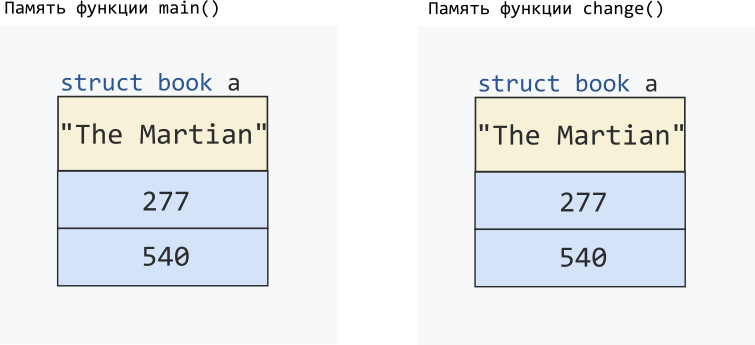
\includegraphics[scale=0.6]{../images/structpassbyvalue.png}
\end{center}


\subsection*{Передача по указателю}
При передаче в функцию по указателю копируется только указатель.
\begin{lstlisting}
#include <stdio.h>
struct book {
    char title[50];
    int pages;
    float price;
};
void change(struct book* p) {
    p->price += 10;
}
int main() {
    struct book a = {"The Martian",277,540};
    struct book* p = &a;
    change(p);
}
\end{lstlisting}
\begin{center}
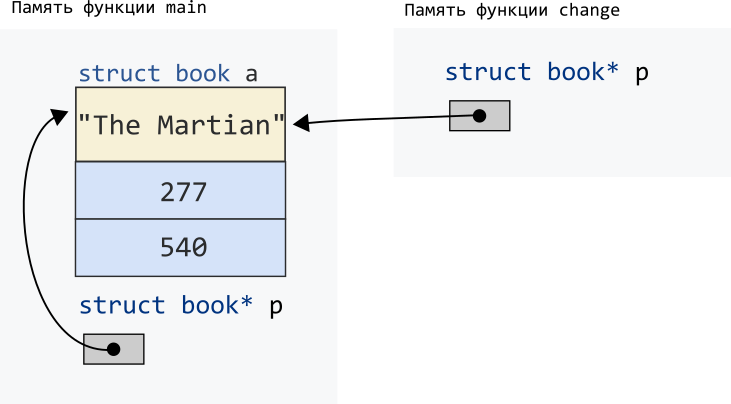
\includegraphics[scale=0.6]{../images/structpassbypointer.png}
\end{center}
Такой способ передачи имее 2 преимущества:
\begin{enumerate}
\item Можно менять структуру внутри функции, и изменения будут действительны вне функции
\item Не приходится копировать структуры, поэтому программа работает быстрее.
\end{enumerate}

\subsection*{Передача по указателю на константу}
Иногда мы не хотим менять структуру внутри функции, но хотим чтобы ничего не копировалось. Тогда желательно использовать передачу по указателю
на константу.
\begin{lstlisting}
#include <stdio.h>
struct book {
    char title[50];
    int pages;
    float price;
};
void print_book_info(const struct book* p) {
    printf("Title: %s\nPages: %d\nPrice: %g\n\n", p->title, p->pages, p->price);
}
int main() {
    struct book a = {"The Martian",277,540};
    change(&a);
}
\end{lstlisting}
\newpage


\begin{itemize}
\item Создать указатель \texttt{struct movie*} и присвоить ему адрес переменной типа \texttt{struct movie}.  Изменить поле \texttt{running\_time}, используя только указатель.  Используйте либо оператор точка (\texttt{.}) и оператор стрелочка (\texttt{->}).
\item Написать функцию \texttt{change\_rating(struct movie* pm, float new\_rating)} и вызвать её в функции \texttt{main}.


\item \textbf{Поиск лучшего фильма:} Написать функцию, которая принимает на вход массив фильмов и возвращает указатель на фильм с самым высоким рейтингом. Протестируйте в функции \texttt{main}.

\item \textbf{Считывание:} Написать функцию \texttt{scan\_movie(struct movie* m)} и вызвать её в функции \texttt{main}. Функция должна считывать фильм  из стандартного входа с помощью \texttt{scanf} (каждое поле нужно считать отдельно).

\end{itemize}


\newpage
\section*{Часть 4: Выравнивание}
Пусть есть структура \texttt{struct test} и нам нужно узнать её размер если размеры типов \texttt{char}, \texttt{int} и \texttt{double} равны \texttt{1}, \texttt{4} и \texttt{8} байт соответственно.
\begin{lstlisting}
struct test {
    int a;
    char b;
    double c;
};
\end{lstlisting}
Кажется, что размер этой структур равен сумме размеров состовляющих её элементов, то есть \texttt{13}. Но это не так. 
На самом деле размер этой структуры будет отличаться в зависимости от вычислительной системы, на которой запускается код (как, впрочем, и размеры других типов). Но на большинстве вычислительных систем размер структуры \texttt{struct test} будет больше суммы состовляющих её элементов. Это можно проверить с помощью следующего кода:


\begin{lstlisting}
int main() {
    printf("Size of char   = %llu\n", sizeof(char));
    printf("Size of int    = %llu\n", sizeof(int));
    printf("Size of double = %llu\n", sizeof(double));
    printf("Size of test   = %llu\n", sizeof(struct test));
}
\end{lstlisting}

Причина по которой это происходит заключается в том, что система значительно быстрей работает с данными, если они лежат в памяти по адресам, кратным 4-м или 8-ми. Поэтому компилятор автоматически выравнивает элементы структуры в памяти так, чтобы их адреса были кратны некоторой степени двойки.

Проверьте чему будет равен размер структуры \texttt{struct test} в зависимости от последовательности её полей.


\iffalse
\newpage
\section*{Справочная информация по указателям:}
Каждая переменная в языке C хранится где-то в памяти и имеет адрес. Адрес переменной это просто номер первого байта соответствующей области памяти. Чтобы получить адрес переменной нужно перед переменной поставить \&(амперсанд).
Указатель это переменная, которая хранит адреса переменных. Тип указателя такой: <тип переменной>*. Пример:
\begin{lstlisting}
int a = 42;  // Переменная, которая хранит число 42
int* address_of_a = &a; // Указатель, который будет хранить адрес переменной a
\end{lstlisting}
Чтобы доступиться к переменной по указателю нужно поставить символ * перед указателем\\
\texttt{a} и \texttt{*address\_of\_a} это абсолютно одно и то же. \texttt{a  ==  *address\_of\_a}.
\begin{lstlisting}
*address_of_a = *address_of_a + 10;
printf("%d", a);  // Напечатает 52
printf("%d", *address_of_a); // Напечатает 52
\end{lstlisting}
Указатели часто используются чтобы изменять передаваемые значения в функциях:
\begin{multicols}{2}
\begin{lstlisting}
// Неправильно:
void normalize(float x, float y)
{
    float sum = x + y;
    x = x / sum;
    y = y / sum; 
    // Изменятся x и y - копии a и b
}
// ...
float a = 20.0, b = 80.0;
normalize(a, b);
// a и b не изменятся: a=20.0, b=80.0
\end{lstlisting}
\begin{lstlisting}

// Правильно:
void normalize(float* px, float* py)
{
    float sum = *px + *py;
    *px = *px / sum;
    *py = *py / sum; 
    // Изменятся переменные a и b
}
// ...
float a = 20.0, b = 80.0;
normalize(&a, &b);
// a и b изменятся:a=0.2, b=0.8
\end{lstlisting}
\end{multicols}
\section*{Типы передачи в функцию:}
\begin{enumerate}
\item По значению. То что передаётся в функцию копируется. При изменении копий, оригинал не меняется.
\begin{lstlisting}
void func(int a)
\end{lstlisting}
\item По указателю. В функцию копируется адрес переменной. Используя этот адрес, можно изменить оригинал.
\begin{lstlisting}
void func(int* p)
\end{lstlisting}
\item По постоянному указателю. В функцию копируется адрес переменной, но изменять оригинал с помощью этого указателя запрещено. Используется для того чтобы передать в функцию переменую большого размера (например структуру) и если вы не хотите изменять её внутри функции. Помогает избежать лишнего копирования.
\begin{lstlisting}
void func(const int* p)
\end{lstlisting}
\end{enumerate}
\fi
\end{document}